\chapter{Methods} \label{sec:methods}

\section{Subjects} \label{methods:subjects}
All experimental procedures were approved by the Harvard Medical School Institutional Animal Care and Use Committee and were performed in compliance with the Guide for the Care and Use of Laboratory Animals. Data were acquired from five male C57BL/6J mice (Jackson Labs), which were 8-10 weeks old at the start of behavioral training, and 14-22 weeks old during imaging. Prior to training, a titanium headplate was affixed to the mouse’s skull using dental cement (Metabond, Parkell). Mice were placed on a water schedule, in which they received 800 μl of water each day (total, including rewards).  Each mouse’s weight was measured daily to ensure that it was  80\% of the mouse’s pre-water-restriction weight.  

\section{Imaging} \label{methods:imaging}
\subsection{Surgical procedure} \label{methods:surgery}
When mice performed well on maze 7 (Figure \ref{fig:2_3}), they underwent a surgery (isoflurane anesthesia) to implant a cranial window. For three days prior to surgery, mice were given 5 mL of water per day. The behavioral training headplate was removed, and a circular craniotomy with a diameter of 3.1 mm was made over PPC on the left hemisphere (stereotaxic coordinates: 2 mm posterior, 1.75 mm lateral of bregma). A virus mixture containing a 4:1 volumetric ratio of tdTomato (AAV2/1-\textit{CAG}-tdTomato) to GCaMP6 (AAV2/1-\textit{synapsin-1}-GCaMP6f or AAV2/1-\textit{synapsin-1}-GCaMP6m) was delivered by three injections of $\sim$20 nL ($\sim$5 min/injection, $\sim$150 μm spacing between injections). Viruses were obtained from the University of Pennsylvania Vector Core Facility. Injections were made near the center of the craniotomy, $\sim$275 μm below the dura, using a beveled glass pipette ($\sim$15 μm tip diameter) and a custom air pressure injection system. The pipette was advanced using a micromanipulator (Sutter MP285) at a 30-degree angle to minimize compression of the brain. A window with glass plug (5 mm diameter coverslip plus two 3 mm diameter coverslips; \#1 thickness; CS-3R and CS-5R, Warner Instruments) was made using UV-curable optically transparent adhesive (Norland Optics). The window was affixed to the brain using a drop of Kwik-Sil (World Precision Instruments) and affixed to the skull using Metabond mixed with  5\% vol/vol India ink, to prevent light leakage. A headplate was affixed to the skull using Metabond mixed with India ink. A titanium ring was mounted on top of the headplate to interface with a cylinder of black rubber to surround the microscope’s objective lens, thus preventing light leak from the VR display into the microscope \citep{Dombeck:2010jr}. Following at least one day of recovery, mice resumed training. Imaging began at least 4 weeks post-injection and was continued for up to 12 weeks. Fields-of-view containing cells with GCaMP6 in the nucleus were excluded. In a given session, we imaged 350 neurons simultaneously during 300 trials (range, 188-648 neurons; range, 231-414 trials; n = 5 mice; Figure \ref{fig:3_2}).

\subsection{Two-photon microscope design} \label{methods:microscope}
Imaging was performed using a custom-built two-photon microscope. The microscope scan head included a resonant scanning mirror and a galvanometric mirror separated by a scan lens-based relay telescope. Fluorescence light collection optics were based on a custom design to collect wide dispersion angles from large (20 mm) back aperture objectives. Collection optics were housed in an aluminum box to prevent light interference from the VR display. The microscope was stationary, and the mouse was mounted on an XYZ translation stage (Dover Motion). Green and red emission light were separated by a dichroic mirror (580 nm long-pass, Semrock) and bandpass filters (525/50 and 641/75 nm, Semrock) and collected by GaAsP photomultiplier tubes (Hamamastu). Excitation light was delivered from a Ti:sapphire laser (Chameleon Vision II, Coherent) operated at 920 nm. The microscope was controlled by ScanImage (version 5; Vidrio Technologies) \citep{Pologruto:2003bq}.

\subsection{Imaging data acquisition} \label{methods:data_acq}
Imaging data were acquired at 30 Hz at a resolution of 512 x 512 pixels ($\sim$700 μm x $\sim$700 μm field-of-view) using a Nikon 16x 0.8 NA objective lens. Imaging and behavioral data were synchronized using custom-written MATLAB software by simultaneously recording the frame clock from Scanimage and an iteration counter from ViRMEn. Imaging data were acquired in sets of 25,000 frames with brief breaks between acquisitions to ensure alignment of the scans. Up to 100,000 frames were acquired from each imaging session over the course of $\sim$1 hour. Imaging data were acquired from single planes at depths between 100 and 200 μm below the dura. Multiple fields-of-view were acquired from the same mouse across different days. Data were analyzed from 11 fields-of-view from 5 mice. 

\subsection{Pre-processing of imaging data} \label{methods:preprocessing}
Motion correction, the definition of putative cell bodies, and extraction of fluorescence traces (\textit{$\Delta$F/F}) were performed in a semi-automatic fashion using custom-written MATLAB software (manuscript in preparation). In brief, following motion correction \citep{Greenberg:2009gn}, the correlation of fluorescence timeseries was calculated for each pair of pixels within 60 μm of one another. Fluorescence sources (putative cells) were then identified by applying a continuous-valued, eigenvector-based approximation of the normalized cuts objective \citep{Shi:2000gf} to the correlation matrix, followed by discrete segmentation by k-means clustering, yielding binary masks for all identifiable fluorescence sources. For each putative cell, the local neuropil fluorescence was estimated by averaging across nearby pixels devoid of fluorescence sources. The scale of neuropil contamination of the cell fluorescence was estimated by regressing the background timeseries against low-activity regions of the cell timeseries, and the scaled background timeseries was then subtracted from the cell timeseries. Cell selection and neuropil subtraction were performed using a tool that allowed manual examination of clustering results and parameters, in combination with anatomical information and fluorescence traces corresponding to each cluster. All neuropil contamination fits were also examined by eye and adjusted when necessary. All fluorescence traces were deconvolved to estimate the probability of a spike in each frame (estimated spike count) \citep{Vogelstein:2010jl}, which minimized the impact of the indicator’s decay kinetics on our analyses. Similar results were obtained from the non-deconvolved \textit{$\Delta$F/F} traces (Figure \ref{fig:3_16}).

\section{Data analysis} \label{methods:data_anal}
\subsection{General analysis procedures} \label{methods:general_anal}
Data were grouped into spatial bins (3.75 cm/bin) corresponding to locations in the virtual maze. To bin data from positions in the arms of the T-maze, the T-maze was linearized prior to binning by folding the arms such that they were a continuation of the stem. Neuronal activity and behavioral parameters were averaged in each bin. On average, each bin contained 2-3 imaging frames per trial. Unless otherwise noted, all analyses were performed on both correct and error trials together. All correlation coefficients were from Pearson’s correlations. Portions of this research were conducted on the Orchestra High Performance Compute Cluster at Harvard Medical School. This NIH supported shared facility consists of thousands of processing cores and terabytes of associated storage and is partially provided through grant NCRR 1S10RR028832-01.

\begin{FPfigure}
%\begin{figure}
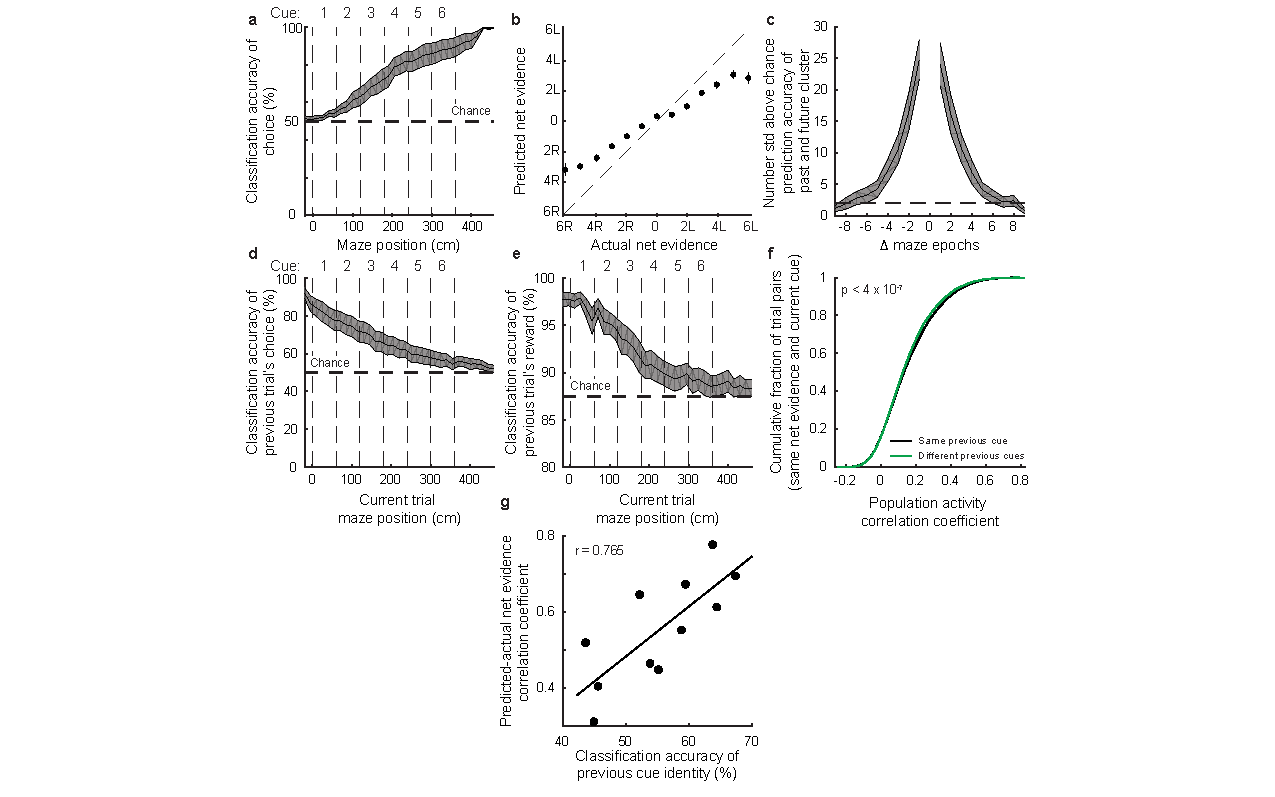
\includegraphics[width=1.6\textwidth,center]{figures/fig_3_16.pdf}
\caption[Main results re-analyzed using $\Delta$F/F values.]
{\textbf{Main results re-analyzed using $\Delta$F/F values. a,} Classification accuracy for choice as a function of maze position (SVM, radial basis function kernel). Independent classifiers were trained and tested at each maze position. Error bars represent mean $\pm$ s.e.m. across datasets. Compare to Figure \ref{fig:3_3}e. 
%
\textbf{b,} Actual net evidence vs. net evidence predicted by a SVR classifier. Error bars represent mean $\pm$ s.e.m. across datasets. Compare to Figure \ref{fig:3_3}f. 
%
\textbf{c,} For a given trial based on the current epoch's cluster identity, the accuracy of predicting the clusters occupied by that trial in the past and future epochs, compared to shuffled assignments of trials to clusters. Error bars represent mean $\pm$ s.e.m. across datasets. Compare to Figure \ref{fig:3_9}e. 
%
\textbf{d-e,} Classification accuracy as in (\textbf{a}), but for previous trial's choice and for whether the previous trial was rewarded (\textbf{e}). Compare to Figure \ref{fig:3_12}b-c. 
%
\textbf{f,} Cumulative distribution of the pairwise trial-trial population activity correlation coefficients for trials with the same (black) or different (green) previous cues given the same maze epoch and same net evidence (p < 4 x 10-7, two-sample KS test). Compare to Figure \ref{fig:3_15}a. 
%
\textbf{g,} Relationship between classification accuracy of the previous cue and the classification accuracy of net evidence across datasets (r = 0.76, p < 0.001). Compare to Figure \ref{fig:3_15}b.
\label{fig:3_16}}
%\end{figure}
\end{FPfigure}
\clearpage

\subsection[Choice selectivity for individual neurons]{Choice selectivity for individual neurons (Figure \ref{fig:3_3}a-c)} \label{methods:choice_sel}
Normalized activity was calculated for each neuron individually by dividing its estimated spike count within each bin on each trial by its maximum across all bins of all trials (Figure \ref{fig:3_3}a-b). To calculate the left-right choice selectivity index (Figure \ref{fig:3_3}c), for each neuron individually, we calculated its average activity for each spatial bin separately across left 6-0 trials and right 0-6 trials. The selectivity index was defined as:

\vspace*{-30pt}

\begin{equation*}
\textrm{Selectivity index} = \frac{\mu_{left 6-0} - \mu_{right 0-6}}{\mu_{left 6-0} + \mu_{right 0-6}}
\end{equation*}

A selectivity index of +1 corresponds to a neuron which is active exclusively on left 6-0 trials, while a selectivity index of -1 corresponds to a neuron which is active exclusively on right 0-6 trials. A selectivity index of 0 corresponds to a neuron with equivalent mean activity in both conditions. The selectivity index for each neuron was calculated separately for each spatial bin, and the peak selectivity index was calculated as the maximum of the absolute value of the selectivity index across all bins. For the shuffled distribution, we shuffled the trial labels (i.e. which trials were left 6-0 or right 0-6), and recalculated the selectivity index as above. 

\section{Classifiers (without clustering)} \label{methods:class_no_cluster}

\subsection[General procedures]{General procedures (Figures \ref{fig:3_3}e-h, \ref{fig:3_5}c, e-h, \ref{fig:3_12}b-d, \ref{fig:3_13})} \label{methods:class_no_cluster_general}

Unless otherwise noted, all population classifiers were support vector machines (SVMs) with a radial basis function (Gaussian) kernel \citep{Murphy:2012uq, Smola:1997uw}. All population classification was performed on the concatenated activity of all individual neurons. All SVMs were implemented using the MATLAB interface of the open-source libsvm library (version 3.20) \citep{Chang:2011ta}. Data were divided into non-overlapping training/validation and test sets (50\% of trials each). To prevent overfitting, models were trained exclusively on the training/validation set, with the test set left untouched until final testing. Hyperparameter (C and γ; regularization weight and radial basis function width, respectively) selection was performed using a random search method with 10-fold cross-validation on the training/validation set of only a single dataset, and the same hyperparameters were used for all datasets. For classifiers applied to the activity of individual neurons (Figure \ref{fig:3_3}d), classifiers were trained with the activity of the given neuron as the only input feature. For population classifiers (Figures \ref{fig:3_3}e-h, \ref{fig:3_5}c, e-h, \ref{fig:3_12}b-d, \ref{fig:3_13}), the activity of all neurons in the population were used as the input to the SVM.

\subsection[Two-class classifications]{Two-class classifications (Figures \ref{fig:3_3}e, g, \ref{fig:3_5}c, \ref{fig:3_12}, \ref{fig:3_13} \ref{fig:3_16}a, d-e)} \label{methods:two_class_classifications}
For two-class classification problems, such as the classification of the choice (Figures \ref{fig:3_3}e, g, \ref{fig:3_5}c), previous trial’s choice (Figure \ref{fig:3_12}b), and previous trial’s reward outcome (Figure \ref{fig:3_12}c), a C-Support Vector Classification (C-SVC) approach was used. Independent SVMs were trained on each spatial bin. In cases where classification accuracy based on neuronal data was compared with accuracy based on behavioral data (Figure \ref{fig:3_13}), hyperparameters were optimized separately for each. 

\subsection[Multi-class classifications]{Regression for net evidence (Figures \ref{fig:3_3}d, f, h, \ref{fig:3_5}e-h, \ref{fig:3_16}b)} \label{methods:multi_class_classifications}
For the regression of net evidence (Figures \ref{fig:3_3}d, f, h, \ref{fig:3_5}e-h), an $\epsilon$-Support Vector Regression ($\epsilon$-SVR) approach was used to obtain a continuous approximation of net evidence \citep{Murphy:2012uq, Smola:1997uw, Chang:2006bj}. For the net evidence models, the average activity during the third quarter of each cue’s presentation ($\sim$200 ms) was calculated for each neuron. For training and testing, each cue was treated as a separate trial with class labels corresponding to the net evidence including that cue. Training and testing sets were divided based on whole trials to prevent similar activity on different cues within the same trial from corrupting the results. To determine prediction accuracy, the predicted class label was compared to the actual class label via a correlation coefficient. To calculate statistical significance, the results were compared to the distribution resulting from 1000 shuffles of class labels. To rule out categorization, which would result in identical guesses within left and right net evidence conditions, but a positive slope across all net evidence conditions, we calculated significance separately within left and right net evidence conditions; both were statistically significant across mice for the population classifiers (p < 0.001; Figure \ref{fig:3_3}f). To exclude the impact of view angle alone, which changes the visual scene, on net evidence classification, we recalculated the $\epsilon$-SVR separately for left and right trials with nearly identical view angles ($\pm$2.5\textdegree; Figure \ref{fig:3_5}e-f). To exclude the impact of view angle in conjunction with other behavioral parameters, such as the x/y position in the maze and the rotational velocity of the spherical treadmill, we trained SVR classifiers to predict net evidence based on either behavioral parameters alone or behavioral parameters in addition to neuronal population activity (Figure \ref{fig:3_5}g-h).

\subsection[Classifiers built by adding-in subsets of neurons]{Classifiers built by adding-in subsets of neurons (Figure \ref{fig:3_3}g-h)} \label{methods:addin}
Classifiers were built similar to the population classifiers described in Methods \ref{methods:class_no_cluster_general}, except with the input being a subset of neurons. The single neuron choice selectivity and SVR net evidence correlation were used to determine single neuron selectivity for choice and net evidence, respectively. Neurons were sorted in ascending order based on their selectivity. A separate classifier was trained for increasingly larger populations of neurons with neurons added in from least to most selective. 


\subsection[Classification of cue sequences]{Classification of cue sequences (Figures \ref{fig:3_5}d, \ref{fig:3_15}a-b, \ref{fig:3_16}g-h)} \label{methods:cue_seq_classifier}

To determine if the identity of previous cues could be read out at a current epoch, given identical current cue and net evidence (Figures \ref{fig:3_5}d, \ref{fig:3_15}a-b), we examined pairwise trial-trial population activity correlations. At each of cues 3-6, we separated trial into those which contained the patterns \textit{LRL} (left-right-left) and \textit{RLL} (right-left-left) or \textit{LRR} and \textit{RLR} with the last cue in the pattern matching the currently analyzed cue. For example, at the third cue, the pattern \textit{LRLRRR} would be a match, while at fifth cue, the pattern \textit{RRLRLR} would be a match. To rule out predictability due to differences in net evidence, a subset of trials in which the distribution of net evidence was equivalent across the two groups was used. This procedure resulted in eight groups (2 choices x 4 patterns). At each cue epoch, pairwise trial-trial correlations of the mean neuronal population activity vector for \textit{n} simultaneously imaged neurons were calculated for trials with the same previous cue or different previous cues. To predict the previous cue based on these correlations, in a leave-one-out fashion, the mean population activity correlations between the test trial and all other trials with a left or right previous cue were calculated; whichever previous cue had a higher correlation with the test trial was considered the prediction of the classifier. To determine significance, accuracy was compared to the distribution of accuracies resulting from 1000 shuffles of the labels assigning previous cues to trials. 

\section{Analysis of activity in high-dimensional state space }  \label{methods:high_d}

\subsection[Factor analysis]{Factor analysis (Figures \ref{fig:3_12}a, \ref{fig:3_14})} \label{methods:factor_analysis}
For visualizations using factor analysis (Figures \ref{fig:3_12}a, \ref{fig:3_14}), dimensionality was reduced to 5-factors using built-in MATLAB toolboxes. Two factors were selected from these five for visualization.  


\subsection[Relationship between pairwise trial-trial distances before and after cue presentation]{Relationship between pairwise trial-trial distances before and after cue presentation (Figure \ref{fig:3_10}a-b)} \label{methods:offset}

To calculate the correlation between the distance between trials before and after a cue(s) (Figure \ref{fig:3_10}a-b), trials were divided into groups based on the number of cues presented between measurements (e.g. $\Delta$2 cues is equivalent to measuring before the first cue and after the second cue or measuring before the third cue and after the fourth cue). Within each group, only trials with the same marginal cues and starting net evidence were compared. The Euclidean distance in n-dimensional activity space between pairs of trials was calculated before (pairwise starting distance) and after (pairwise ending distance) the marginal cues were presented. Across all pairs of trials within each group, the Pearson correlation coefficient of the population activity on each trial was calculated. To determine significance, we generated new ending states for each trial by shuffling the distribution of vectors which define the change in activity in response to cues and adding them to the original starting states. Vectors were calculated by subtracting the n-dimensional vector corresponding to the starting state from the vector corresponding to the ending state. This step was necessary to rule out the possibility that the network activity changed little in comparison to the original distance between trials. For example, if two trials were separated by a distance of 10 estimated spikes, but the activity only changed by 0.1 estimated spikes, the pairwise ending distance would be expected to remain strongly correlated with the pairwise starting distance, regardless of the direction of the vectors. A p-value was then calculated by comparing the correlation coefficient to the distribution obtained from 1000 such shuffles.

\subsection[Relationship between pairwise trial-trial distances and population activity vectors]{Relationship between pairwise trial-trial distances and population activity vectors (Figure \ref{fig:3_10}c-d)} \label{methods:vector}

To calculate the correlation between the distance between trials before the presentation of a cue and the vector which results from the response to the cue (Figure \ref{fig:3_10}c-d), trials were divided into groups and paired in the same fashion as described above. Vectors were calculated as described above. For each pair of trials, the similarity between vectors was calculated by determining the Euclidean distance between the two vectors. Across all pairs of trials within each group, the Pearson correlation coefficient between the pairwise starting state distance and the pairwise vector distance was then calculated. Significance was determined by comparing the correlation coefficient to the distribution obtained from 1000 shuffles of the vector trial identities. 


\section[Clustering methods]{Clustering methods (Figures \ref{fig:3_6}, \ref{fig:3_7}, \ref{fig:3_8}, \ref{fig:3_9}, \ref{fig:3_11} \ref{fig:3_15}c, \ref{fig:3_16}c, f)} \label{methods:clustering_general}

We used clustering to reduce the dimensionality of the population activity in as unbiased a fashion as possible, without inclusion of information about behavioral parameters and without encouraging projection of the data onto dimensions which maximize variance due to specific task features, such as choice. We used clustering because it did not assume linearity in the data structure and facilitated analyses by discretizing activity patterns, allowing for the calculation of transition probabilities between discrete activity states. However, clusters were not considered an indication of discreteness of the underlying activity patterns. Clustering revealed groups of trials with similar population activity patterns (Figure \ref{fig:3_6}a-c). 

\subsection{Pre-processing for clustering} \label{methods:clustering_preprocessing}
Prior to clustering, each spatially binned trial was divided into ten non-overlapping epochs, corresponding to the start of the trial, cues 1-6, the early and late delay, and the turn. For the trial-start epoch, neuronal activity was averaged over the 4 spatial bins (15 cm) immediately preceding onset of the first cue. For cues 1-6, activity was averaged over the third quarter of each cue’s presentation (4 spatial bins). For the early and late delay, respectively, activity was averaged across the 4 spatial bins beginning 15 and 37.5 cm after offset of the final cue. For the turn, activity was averaged across the final 4 spatial bins in the maze. Each epoch corresponded to approximately 200 ms.

\subsection{Clustering via affinity propagation} \label{methods:clustering_affinity}
Within each epoch, trials were clustered into groups based on their neuronal activity using affinity propagation \citep{Frey:2007tj}. Affinity propagation has two inputs: a distance matrix and a ‘preference’ for each data point. We calculated the distance as the negative sum of pairwise Euclidean distance and one minus the pairwise cosine similarity between every trial in the n-dimensional activity space (each dimension is the activity of a single neuron). In contrast to other clustering methodologies, such as k-means clustering, the preference parameter does not specify the number of clusters, but rather a general range. For example, in our experience, clustering on different datasets using the same preference parameter can result in anywhere from 1 to 30 clusters. To determine the preference parameter, we calculated the number of clusters generated across a range of preference parameter values. The tenth percentile of the difference matrix was within a stable range, such that small modifications in the preference parameter did not greatly influence the number of clusters identified. The choice of this parameter and the resulting number of clusters had little impact on our results (Figure \ref{fig:3_7}g). Clustering was only used for analyses in which dimensionality reduction was necessary. Affinity propagation was performed using code provided by the laboratory of Brendan Frey.

\subsection[Transition probabilities between clusters]{Transition probabilities between clusters (Figures \ref{fig:3_6}, \ref{fig:3_7}, \ref{fig:3_9})} \label{methods:clustering_trans_prob}

To calculate transition probabilities between clusters at different maze epochs (cluster \textit{a} at epoch 1, cluster \textit{b} at epoch 2), we calculated the fraction of trials in cluster \textit{a} which were also in cluster \textit{b}. To superimpose behavioral variables on clusters (Figures \ref{fig:3_6}e-h, \ref{fig:3_9}a-c), for each cluster, we calculated the fraction of trials that had a given feature. For example, to superimpose left choice probability, we calculated the fraction of trials in each cluster that resulted in a left choice. To validate that the clustering found meaningful groups, we analyzed whether the distribution of behavioral variables across clusters at a given epoch was significantly different than chance. To calculate chance, we shuffled the cluster labels such that the number of trials in each cluster was maintained, but with the trials assigned to a given cluster determined randomly (Figure \ref{fig:3_7}a-d). Significance was established by summing the absolute difference in behavioral variables from the expected uniform distribution for the real data and comparing this total difference to the distribution of the same metric obtained from 1000 shuffles (Figure \ref{fig:3_7}b, d). To determine whether there was a relationship between the similarity of clusters at adjacent epochs and the transition probability between them, for each pair of adjacent clusters, we calculated the mean pairwise trial-trial population activity correlation and compared it to the transition probability (as defined above). Transitions were not significantly more likely between more similar clusters (r = 0.02, p > 0.05).

\subsection[Clustering based on all time points together (rather than epoch-by-epoch clustering)]{Clustering based on all time points together (rather than epoch-by-epoch clustering) (Figures \ref{fig:3_6}l, \ref{fig:3_7}f)} \label{methods:clustering_together}

To determine if clustering separately at each epoch resulted in multiple clusters with similar population activity patterns in different epochs, we also performed clustering on all epochs together. While the total number of clusters for epoch-by-epoch-based clustering was larger than those for all-epoch-based clustering (ratio: 1.6  $\pm$ 0.06), the ratio was relatively low, suggesting that activity patterns were distinguishable across epochs. Self-transitions were identified as transitions across epochs in the all-epoch clustering in which a trial was in the same cluster at two consecutive epochs (Figure \ref{fig:3_7}f). To determine whether the variability of trials in cluster space changed over the course of a trial, we also calculated the fraction of the total clusters explored at each maze epoch (Figure \ref{fig:3_6}l). To remove outliers, only clusters containing three or more trials at a given epoch were counted as visited.

\section{Classifiers based on activity in cluster-space} \label{methods:clustering_classifiers}

\subsection[Classification of the cluster identity at past and future epochs based on the cluster identity at the current epoch]{Classification of the cluster identity at past and future epochs based on the cluster identity at the current epoch (Figures \ref{fig:3_7}k, \ref{fig:3_9}d-e, \ref{fig:3_15}c, \ref{fig:3_16}c)} \label{methods:clustering_past_future_class}

To predict the past or future cluster identity during a trial at a certain epoch (epoch \textit{j}), given the cluster identity at another epoch (epoch \textit{i}), we implemented a classifier built in cluster-space (Figure \ref{fig:3_9}d-e). In a leave-one-out fashion, we limited our analysis to only the trials which were in the same cluster as the test trial at epoch \textit{i}. Of those trials, we then asked which cluster was most common at epoch \textit{j}. The classifier then predicted that the test trial would also be in that cluster at epoch \textit{j}. Prediction accuracy was calculated as the fraction of predicted clusters that matched the actual cluster. In Figure \ref{fig:3_9}d-e, clustering was performed separately on correct left 6-0 and right 0-6 trials to rule out structured variability due to different cues or behavioral choices. Accuracy was calculated across both of these conditions. To establish statistical significance, accuracy was compared to 1000 shuffles of the assignment of trials to clusters. Cluster assignments were shuffled independently at each epoch. This shuffle maintains the distribution of trials across clusters. This classifier was identical to the `cluster only' classifier used in Figure \ref{fig:3_15}c, except in Figure \ref{fig:3_15}c, it was applied to all trials together, independent of evidence or choice. The other classifiers used in Figure \ref{fig:3_15}c followed a similar logic. For the `chance' classifier, the same procedure was followed, except all trials except for the test trial were used to determine the most likely cluster at epoch \textit{j}, not just those in the same cluster at epoch \textit{i}. For the `cue only' classifier, only those trials with the same current cue (left or right) were used to determine the most likely cluster at epoch \textit{j}. For the `cue + cluster' classifier, only those trials with both the same current cue as the test trial and which were in the same cluster at epoch \textit{i} were used to determine the most likely cluster at epoch \textit{j}. 


\subsection[Classification of past and future cluster identities with simulated pseudo-populations ]{Classification of past and future cluster identities with simulated pseudo-populations (Figure \ref{fig:3_7}g)} \label{methods:clustering_pseudopop}

The temporal structure we observed could be caused by the prolonged activity of individual neurons, either due to persistent activity in the underlying neuronal activation or to the prolonged decay kinetics of the calcium indicator. To test if prolonged activity patterns could account for temporally structured and predictable trial-trial variability, we shuffled the trial labels independently for each neuron across trials with the same choice and sequence of evidence cues (e.g. correct left 6-0 trials; Figure \ref{fig:3_7}g). This shuffle therefore breaks neuron-neuron correlation structure, but maintains the temporal structure of each neuron’s individual activity, simulating a pseudo-population. Following this shuffle, clustering was performed (separately for correct 6-0 left and 0-6 right trials), and past and future activity patterns were classified as described above using the `population activity only' classifier. In contrast to the unshuffled case, we were unable to predict past and future activity patterns over more than one epoch (Figure \ref{fig:3_7}g), suggesting that the predictability we observed in the real data could not be explained by prolonged activity or slow indicator kinetics.


\subsection[Classification of past and future cluster identities based on behavioral data]{Classification of past and future cluster identities based on behavioral data (Figure \ref{fig:3_11})} \label{methods:clustering_behav_past_future}

To determine the fraction of past and future predictability accounted for by variability in behavioral parameters across clusters, we used logistic regression to compare predictability based only on behavioral parameters to that based on both behavioral parameters and neuron activity-defined clusters (Figure \ref{fig:3_11}). To allow for binary classification, only trials whose cluster identity contained either the most or second most trials during the prediction epoch were included. We used all recorded behavioral parameters (x/y position, spherical treadmill rotational velocities, view angle) for this analysis, which together account for the mouse’s general running pattern and visual scene. At each epoch, we trained a logistic regression model to predict the activity pattern at the current epoch or at another epoch in the past or the future based on either the behavioral variables alone (behavior only) or the behavioral variables in addition to the current cluster identity (behavior + neuronal activity clusters). Note that for the same epoch, we did not include neuronal clusters as an explanatory variable as they were identical to the response variable in that case. To compare model performance across the two cases, which have different numbers of predictors, we used adjusted R\textsuperscript{2}. Independent models were created for each combination of epochs and combined based on the number of epochs separating the predictor and response (e.g. cue 1 and cue 2 are separated by 1 epoch, while trial start and turn epochs were separated by 9 epochs). Separate models were calculated for left 6-0 and right 0-6 trials to rule out behavioral variability induced by the choice. Results were qualitatively similar when models included linear interaction terms and quadratic terms. 

 

\subsection[Classification of behavioral errors based on cluster identity]{Classification of behavioral errors based on cluster identity (Figures \ref{fig:3_9}g)} \label{methods:clustering_behav_error}

To determine whether behavioral errors were uniformly distributed across clusters (Figure \ref{fig:3_9}g), we clustered trials based on their population activity patterns at the trial start, before any cues had been presented. Because differences in activity were likely to be subtle, we used a conservative clustering approach, which resulted in more clusters. Thus, we used a preference parameter equivalent to the thirtieth percentile of the distance matrix. The distribution of the probability of a behavioral error across these clusters was then calculated. To determine statistical significance, we calculated the expected number of errors in each cluster based on the overall error rate and the number of trials in each cluster and calculated the total absolute difference from the uniform expected error rate in each cluster. This metric was compared to a shuffle of the assignments of trials to clusters.

\section[Analysis of the overlap of active neurons across clusters]{Analysis of the overlap of active neurons across clusters (Figure \ref{fig:3_3}k)} \label{methods:overlap}

To calculate the overlap fraction for active neurons between clusters, each neuron’s activity across all trials was z-scored. Within each cluster, each neuron’s mean z-scored activity was calculated and compared to a z-score activity threshold of 1.5 (Figure \ref{fig:3_3}k), though similar results were obtained using different thresholds. Neurons whose mean z-scored activity was above this threshold were determined to be active. Using correct left 6-0 and right 0-6 trials separately to rule out differences due to evidence cues, the pairwise overlap fraction between all clusters at each epoch was calculated as:

\vspace*{-30pt}

\begin{equation*}
\textrm{Overlap fraction} = \frac{\textrm{number of neurons with activity above threshold in both clusters}}{\textrm{number of neurons with activity above threshold in either cluster}}
\end{equation*}

The mean value across all pairs of clusters at all epochs was calculated. For the intra-cluster measure, trials within a cluster were randomly divided into two groups, the mean activity within each group was calculated for each neuron, compared to the z-score threshold, and the overlap fraction between the two groups was calculated. This process was repeated 100 times and the results were averaged. The mean across all clusters was then calculated. To reduce variability due to low trial numbers, only clusters (intra-cluster measure) or cluster pairs (inter-cluster measure) with greater than 20 combined trials were included. To determine the shuffled overlap fraction, the cell labels within each cluster were randomly assigned 1000 times, and the inter-cluster overlap fraction was recalculated. 
